\documentclass[10pt,twocolumn]{article}

% ============================================
% Optica-like Two-Column Draft Layout
% ============================================

% ===== Page Setup =====
\usepackage[a4paper,margin=0.72in,columnsep=0.24in]{geometry}
\setlength{\parindent}{1em}
\setlength{\parskip}{0pt}

% ===== Basic Packages =====
\usepackage{graphicx}
\usepackage{amssymb,amsthm,amsmath}
\usepackage{xcolor}
\usepackage{hyperref}
\usepackage{booktabs}
\usepackage{array}
\usepackage{natbib}
\usepackage[section]{placeins}
\usepackage{abstract}
\usepackage{titlesec}
\setlength{\emergencystretch}{1.5em}

% ===== Color Setup =====
\hypersetup{
    colorlinks=true,
    linkcolor=blue,
    filecolor=blue,
    urlcolor=blue,
    citecolor=blue
}

\renewcommand{\topfraction}{0.9}
\renewcommand{\bottomfraction}{0.8}
\renewcommand{\textfraction}{0.07}
\renewcommand{\floatpagefraction}{0.8}
\setcounter{topnumber}{3}
\setcounter{bottomnumber}{2}
\setcounter{totalnumber}{5}

% ===== Section Style =====
\titleformat{\section}{\large\bfseries}{\thesection.}{0.5em}{}
\titleformat{\subsection}{\normalsize\bfseries}{\thesubsection.}{0.5em}{}
\titlespacing*{\section}{0pt}{1.0ex plus 0.4ex minus 0.2ex}{0.5ex}
\titlespacing*{\subsection}{0pt}{0.8ex plus 0.3ex minus 0.2ex}{0.4ex}

% ===== Abstract Style =====
\renewcommand{\abstractnamefont}{\normalfont\bfseries}
\renewcommand{\abstracttextfont}{\small}
\setlength{\absleftindent}{0pt}
\setlength{\absrightindent}{0pt}

% ===== Custom Commands =====
\newcommand{\otf}{\textsf{OTF}}
\newcommand{\rcwa}{\textsf{RCWA}}
\newcommand{\tp}{T_{pp}}
\newcommand{\ts}{T_{ss}}
\newcommand{\lam}{\lambda}
\newcommand{\ang}{\theta}
\newcommand{\Rtar}{\mathbf{R}^{\star}}
\newcommand{\Rpred}{\widehat{\mathbf{R}}}
\newcommand{\Rsim}{\mathbf{R}_{\mathrm{sim}}}
\newcommand{\G}{\mathcal{G}}
\newcommand{\D}{\mathcal{D}}
\newcommand{\score}{\mathcal{S}}
\newcommand{\loss}{\mathcal{L}}
\newcommand{\etal}{\textit{et al.}}

\makeatletter
\renewcommand\maketitle{%
  \begingroup
  \renewcommand\thefootnote{\fnsymbol{footnote}}%
  \thispagestyle{plain}%
  \twocolumn[{%
    \centering
    {\Large\bfseries \@title \par}%
    \vspace{0.6em}
    {\normalsize \@author \par}%
    \vspace{0.35em}
    {\footnotesize \@thanks \par}%
    \vspace{0.1em}
    {\small \@date \par}%
    \vspace{0.8em}
    \begin{minipage}{0.92\textwidth}
    \small
    \sloppy
    \begin{abstract}
    Fourier-operator metasurfaces are usually reported task by task, for example as differentiators, edge detectors, angular filters, or polarization-selective processors. Here we focus on Angle-Resolved Fourier-Operator Metasurfaces (AFOM) and propose a general framework for joint wavelength--theta--polarization design and control. In freeform inverse design, the key object to specify and recover is the optical transfer function itself over wavelength, incidence angle, and polarization. This paper rewrites the problem in that form and develops a physics-consistent generative design loop for freeform binary metasurfaces conditioned on the target response tensor. The workflow combines fabrication-aware structure generation, rigorous simulation-based labeling on a two-channel wavelength--angle grid, surrogate-assisted candidate screening, conditional diffusion-based inverse sampling, and simulation-verified reranking under task-specific scores. Within this unified formulation, a large-NA, high-transmission, broadband second-order differentiator is used as the leading benchmark, while polarization-independent, polarization-multiplexed, fourth-order, low-pass, and spatiotemporal targets are treated as controlled variations of the same response-space inverse problem. The results show that this formulation supports high-fidelity verified designs across these diverse targets, with multiple target designs achieving the highest performance among all current designs: second-order cases reach verified task scores above 0.93 across multiple wavelengths, the low-pass benchmark attains a verified score of 0.993, and polarization-independent, polarization-multiplexed, fourth-order, low-pass, and spatiotemporal targets are all successfully realized within the same framework. The main contribution is a response-centered paradigm for metasurface inverse design in which target definition, model training, candidate generation, and final selection remain tied to the verified scattering behavior of the device.

    \vspace{0.5em}
    \noindent\textbf{Keywords:} metasurfaces; inverse design; Fourier optics; angle-resolved response; diffusion model; full-wave simulation; polarization multiplexing
    \end{abstract}
    \end{minipage}
    \vspace{0.8em}
  }]%
  \endgroup
}
\makeatother

\begin{document}

% ===== Title =====
\title{Physics-Consistent Generative Inverse Design of Angle-Resolved Fourier-Operator Metasurfaces}

% ===== Author =====
\author{%
Your Name$^{1}$\thanks{Email: your\_email@example.com} \\
\small $^{1}$School of XXX, University of XXX, City, Country%
}

% ===== Date =====
\date{\today}

\maketitle

% ===== Main Content =====
\section{Introduction}

\subsection{From Fourier optics to angle-resolved operator metasurfaces}

Fourier optics provides the formal language for interpreting imaging systems and linear spatial operators in the frequency domain, where filtering and differentiation are encoded through transfer functions rather than through pointwise geometric manipulations \cite{goodman2017}. In metasurface-enabled analog photonics, this viewpoint has become especially powerful because a subwavelength structured interface can be designed to emulate a desired optical operator within an extremely compact footprint. Recent demonstrations of mathematical metasurfaces and nonlocal operator devices have shown that differentiation, edge enhancement, and polarization-dependent image processing can be implemented by engineering the angular response of nanostructured optical layers \cite{silva2014,cordaro2019,kwon2020,cotrufo2023optica}.

For angle-resolved Fourier-operator metasurfaces, however, the relevant design object is not merely a scalar transmission efficiency or a single transfer-function slice at normal incidence. The device must realize a structured optical response that varies jointly with incidence angle, wavelength, and polarization. This coupled dependence is not a secondary implementation detail; it is the mechanism by which operator fidelity, angular bandwidth, and polarization selectivity are actually realized. Accordingly, a satisfactory inverse-design framework should be able to represent and manipulate the response field itself.

\subsection{Why inverse design remains difficult}

Despite rapid progress in metasurface inverse design, freeform Fourier-operator devices remain challenging because the structure-to-response map is high-dimensional, strongly nonlinear, and frequently non-unique. A large number of distinct binary patterns can yield similar coarse operator behavior while differing substantially in spectral robustness, angular stability, or polarization leakage. Brute-force scanning is therefore prohibitively inefficient, and purely deterministic regression tends to average over valid design modes instead of preserving solution diversity \cite{molesky2018,liu2018,so2019}.

The challenge becomes more pronounced when the target is defined over a multi-axis response field. Conventional design workflows often reduce the problem to one operating wavelength, one incidence condition, or one target task at a time. Such simplifications are useful for isolated demonstrations, but they obscure the central question addressed in this work: whether angle-resolved Fourier-operator metasurface design can be cast as a unified response-space inverse problem whose different practical instantiations emerge from one common formulation.

\subsection{Central thesis and scope of this paper}

The central thesis of this manuscript is that physics-consistent generative inverse design offers a natural framework for this unification. We treat the desired metasurface behavior as a target optical response field $\Rtar(\lam,\ang,p)$ defined over wavelength, incidence angle, and polarization channel. The inverse problem is then to generate one or more physically plausible structures whose verified response matches this target field under full-wave or \rcwa-based evaluation. Under this formulation, second-order differentiation, polarization-multiplexed image processing, and spectrally selective operator behavior are not separate ``tasks'' but different constraints on the same unified response object.

This narrative deliberately avoids framing the work as a platform paper built around a growing library of independent demonstrations. Instead, the paper is organized around a single design paradigm: angle--frequency--polarization response-space engineering enforced through a physics-consistent generative loop. The sections that follow formalize this viewpoint, describe the generative framework, and use representative results to argue that unification is the main scientific contribution.

\section{Methods}

\subsection{Closed-loop framework}

The proposed workflow is organized as a task-driven physical loop in which the generator is embedded within a broader inverse-design pipeline. A target operation is first converted into a task-aware score, and this score quantifies device performance on the desired function while defining the response object used for training, screening, and final reporting. The resulting wavelength--angle--polarization target then drives dataset construction, model training, conditional generation, and final simulation-based reranking. In symbolic form, the workflow can be written as
\begin{equation}
\mathbf{R}^{\star}\xrightarrow{\ \mathcal{S}\ }\mathcal{D}_{\mathrm{train}}
\xrightarrow{\ \mathcal{F},\mathcal{G}\ }\widehat{\mathcal{G}}_{1:K}
\xrightarrow{\ \mathrm{Sim.}\ }\widehat{\mathcal{G}}_{\mathrm{best}},
\end{equation}
where $\mathbf{R}^{\star}$ is the target response tensor, $\mathcal{S}$ denotes the task-specific score family, which converts agreement between the target OTF and device response into a directly comparable task-performance score, $\mathcal{D}_{\mathrm{train}}$ is the simulation-grounded training set, $\mathcal{F}$ is the forward surrogate, $\mathcal{G}$ is the conditional diffusion generator, and $\widehat{\mathcal{G}}_{1:K}$ denotes the generated candidate set. The reported output is determined by the candidate with the best verified simulation score under the chosen task, because the manuscript ultimately reports task performance rather than model-internal preference.

This choice is essential for two reasons. First, the forward and inverse models are trained against the same optical object that is later used for physical verification. Second, the candidate set remains explicit throughout inference, which is necessary because the inverse mapping from response to geometry is multimodal. The role of the forward surrogate is especially important here. The diffusion model does not directly encode electromagnetic response laws; by itself it learns structure-generation patterns from data. The forward surrogate provides an approximate structure-to-response map and injects response-level physical constraints through the surrogate-guided physics loss used during diffusion training. This loss pulls the generative process back toward regions that satisfy the target electromagnetic response, so the sampled candidates are shaped jointly by data priors and physical consistency. The pipeline therefore treats rigorous electromagnetic simulation as the physical source of truth at both training and inference time, while learned models are used to allocate solver effort, populate the feasible set efficiently, and inject response-aware constraints during training.

\subsection{Dataset construction, scoring, and augmentation}

The geometry class is a fabrication-oriented $64\times64$ freeform binary pattern with the convention $1=\mathrm{material}$ and $0=\mathrm{air}$. The structure generator starts from a coarse random field, imposes $C_4+\sigma_x+\sigma_y$ symmetry, and upsamples to the final resolution. This $D_4$-type symmetry prior is introduced to promote in-plane isotropy while retaining freeform flexibility: under this constraint, the structure or angular response over the $0^{\circ}$--$45^{\circ}$ sector is already sufficient to determine the full metasurface by symmetry folding. Two rounds of Gaussian smoothing followed by binarization are then used to progressively form a manufacturable freeform pattern: the first round turns the rough random field into a continuous shape prototype, while the second further regularizes boundaries and suppresses fragmented high-frequency details. To approximately enforce a minimum feature size, the code then applies morphology-based opening and closing operations. The opening step removes small protrusions, isolated islands, and overly thin bridges, whereas the closing step fills small holes and narrow cracks; if the cleanup becomes too aggressive, the procedure falls back to a more conservative closing-only variant. This produces a structure space that goes well beyond a small analytic family while remaining compatible with fabrication-oriented constraints.

All structures are labeled by RCWA under a fixed material stack consisting of a $500$~nm-period silicon patterned layer of thickness $500$~nm, illuminated from air and transmitting into silica. The response grid contains $11$ sampled wavelengths from $800$ to $1300$~nm in $50$~nm steps and $17$ sampled angles from $-40^{\circ}$ to $40^{\circ}$ in $5^{\circ}$ steps. Two polarization-preserving channels are retained, namely $T_{pp}$ and $T_{ss}$ magnitude maps, so each training condition is represented as a tensor of shape $[2,11,17]$. Although compact, this discretization is already sufficient to resolve wavelength drift, angular curvature, and polarization leakage across the operator families considered here.

Let $R_q(\lambda_j,\theta)$ denote the verified response slice of polarization channel $q\in\{p,s\}$ at sampled wavelength $\lambda_j$, and let
\begin{equation}
\widetilde{R}_q(\lambda_j,\theta)=\frac{R_q(\lambda_j,\theta)}{\max_{\theta}R_q(\lambda_j,\theta)+\varepsilon}
\end{equation}
be the row-wise normalized response used for shape comparison. The role of the scoring functional family is to project each physical target onto a verified response criterion that is both task aware and numerically comparable across structures. In that sense, the score does not merely rank candidates after simulation; it acts as the explicit bridge from optical specification to learnable target.

For the second-order differentiator with large NA, high transmission, and broadband operation, the ideal angular envelope is written as
\begin{equation}
g_2(\theta)=\left|\frac{\sin\theta}{\sin\theta_{\max}}\right|^{2},
\end{equation}
and the row-wise score is defined by
\begin{equation}
S_2=(1-\alpha)\left(w_c S_c+w_s S_s+w_e S_e\right)+\alpha S_b.
\end{equation}
Here $S_c$ rewards suppression near $\theta=0$, $S_s$ measures agreement with the target $k_x^2$-like envelope, $S_e$ rewards sufficiently strong outer-angle transmission, and $S_b$ enforces persistence of the same operator behavior at neighboring wavelengths. These four terms correspond respectively to low-spatial-frequency suppression, correct differentiator-like angular growth, preservation of high-spatial-frequency content, and finite-bandwidth robustness. Other task-specific scores are built on the same response-centered principle and are detailed in the Supporting Information.

\subsection{Forward surrogate}

The forward surrogate learns the mapping
\begin{equation}
\mathcal{F}_{\phi}: \mathbf{G}\in\{0,1\}^{64\times64}\mapsto \widehat{\mathbf{R}}\in\mathbb{R}^{2\times11\times17},
\end{equation}
where $\widehat{\mathbf{R}}(:,j,k)$ denotes the joint two-polarization prediction at the $j$th wavelength sample and the $k$th angle sample. Its role is intentionally limited but physically important: it provides a fast approximation to the structure-to-response map for large-scale candidate screening, supplies the response-consistency term used to guide diffusion training, and reallocates RCWA effort toward candidates that are more likely to satisfy the target response.

Architecturally, the model is a coordinate-aware convolutional encoder followed by multiscale response-grid fusion. Two Cartesian coordinate channels are concatenated to the binary geometry so that the network can relate planar layout to angular scattering directionality rather than treating the pattern as a translation-invariant texture. Residual convolutional blocks then encode the structure across progressively coarser scales, which is important because local subwavelength boundaries and global topology influence the response in different ways. Instead of decoding back to the image plane, all feature levels are projected directly onto the $11\times17$ wavelength--angle grid and fused there, so the prediction head operates on the same physical sampling manifold used for RCWA labels.

The deepest latent representation is further compressed by a global multilayer perceptron and broadcast to the whole response grid, injecting device-level information such as overall topology and effective fill into every wavelength--angle location. The response grid itself is also endowed with explicit coordinates, allowing the network to distinguish central from outer angles and short from long wavelengths. Finally, the two polarization-preserving channels are predicted jointly rather than separately, because $T_{pp}$ and $T_{ss}$ originate from the same geometry and their correlation or leakage is itself part of the physical specification.

For training, the response tensor is normalized pointwise across channel, wavelength, and angle, invalid simulation samples are removed before statistics are computed, and augmentation is restricted to symmetry-preserving flips that leave the optical response unchanged. The surrogate is optimized with an $L_1$ loss in normalized response space,

The surrogate is optimized with an $L_1$ loss in normalized response space,
\begin{equation}
\mathcal{L}_{\mathrm{fwd}}=\left\|\mathcal{F}_{\phi}(\mathbf{G})-\widetilde{\mathbf{R}}\right\|_{1},
\end{equation}
while physical-space MAE is tracked during validation after denormalization. In the retained training log, the normalized validation loss decreases from about $0.63$ at initialization to about $0.366$ near the end of training, which is sufficient for the model to act as a practical screening oracle even though final claims are still deferred to full-wave simulation.

\subsection{Conditional diffusion inverse design}

The inverse model is a conditional diffusion process that takes the target response tensor as condition and samples binary structure candidates. During training, binary layouts are remapped from $[0,1]$ to $[-1,1]$, a cosine noise schedule is used, and the model is trained in the velocity parameterization $v$. Let $x_0$ denote the clean structure, $x_t$ the noisy sample at time step $t$, and $\mathbf{c}$ the normalized target response tensor. The forward noising process is
\begin{equation}
x_t=\sqrt{\bar{\alpha}_t}\,x_0+\sqrt{1-\bar{\alpha}_t}\,\epsilon,\qquad \epsilon\sim\mathcal{N}(0,I),
\end{equation}
and the network learns $v_{\theta}(x_t,t,\mathbf{c})$ under a diffusion loss
\begin{equation}
\mathcal{L}_{\mathrm{diff}}=\left\|v_{\theta}(x_t,t,\mathbf{c})-v^{\star}(x_0,\epsilon,t)\right\|_2^2.
\end{equation}

The backbone is a conditional U-Net with three design choices that are particularly important for this problem. First, the condition is itself a structured two-channel response field, so the model uses a dedicated condition encoder in place of a simple class-label embedding. This encoder maps the target tensor into a global condition embedding, a hierarchy of condition feature maps, and a set of spectral tokens, so the same response specification is available in both compact and spatially structured forms. Second, the global embedding is injected into residual blocks together with the time embedding, while the condition feature maps are fused into the corresponding decoder and encoder resolutions; in parallel, cross-attention injects the spectral tokens into the latent spatial hierarchy, allowing local geometry evolution to remain coupled to the global wavelength--angle response pattern throughout denoising. Third, classifier-free guidance is enabled by condition dropout during training and by guided sampling during inference.

Pure diffusion loss is not enough for this application, because a visually plausible binary layout can still be physically poor. The training objective therefore adds two auxiliary terms:
\begin{equation}
\mathcal{L}_{\mathrm{total}}
=\mathcal{L}_{\mathrm{diff}}
+\lambda_{\mathrm{phys}}\mathcal{L}_{\mathrm{phys}}
+\lambda_{\mathrm{bin}}\mathcal{L}_{\mathrm{bin}},
\end{equation}
where $\mathcal{L}_{\mathrm{phys}}=\|\mathcal{F}_{\phi}(\widehat{x}_0)-\mathbf{c}\|_1$ encourages the denoised prediction to preserve the target response under the forward surrogate, and $\mathcal{L}_{\mathrm{bin}}$ penalizes uncertain gray values through $x(1-x)$. In this formulation, $\mathcal{L}_{\mathrm{phys}}$ is the mechanism that injects response-level physical constraints into diffusion training through the surrogate-predicted electromagnetic behavior. In the retained training setup, $\lambda_{\mathrm{phys}}=0.5$ and $\lambda_{\mathrm{bin}}=0.05$. The final saved validation loss is around $0.129$, with the physics term remaining a nontrivial contributor throughout training. This supports the interpretation that the inverse model is being pushed toward physically meaningful candidates instead of merely toward dataset likeness.

\subsection{Physics-guided inference and simulation-based reranking}

Inference is deliberately candidate-based. For each target case, an ideal target OTF over $(\lambda,\theta,p)$ is constructed, normalized with the saved statistics, and repeated $K$ times to condition batch sampling. The diffusion model then produces multiple binary candidates with classifier-free guidance. The surrogate supplies an inexpensive first-pass ranking, after which selected candidates are pushed back through full-wave simulation under the exact wavelength and angle points relevant to the task.

The final metric is task specific but always evaluated in verified response space. For example, the second-order score combines center suppression, agreement with the ideal even-symmetric angular profile, and outer-angle support. The polarization-independent score adds channel matching. The polarization-multiplexed score rewards the active channel while suppressing the passive one. The spatiotemporal score evaluates the full wavelength--angle window instead of a single row. This division of labor is the practical definition of physics consistency in the paper: neural models generate and pre-rank candidates, while verified scattering responses determine what is ultimately reported as the design outcome.

\section{Results}

\subsection{Second-Order Differentiators with Large NA, High Transmission, and Broadband Operation}

This second-order benchmark is emphasized here because it simultaneously requires large numerical aperture, high transmission, broadband operation, response curvature control, center suppression, outer-angle support, and practical image-processing behavior. The verified second-order score is evaluated wavelength by wavelength on the $T_{pp}$ response row. The resulting score landscape is highly nonuniform, with mean scores around $0.15$--$0.17$ over the full dataset but top candidates rising above $0.93$ at 1050 and 1100~nm. This gap is important: it shows that the feasible set is sparse but not empty, exactly the regime in which generative candidate exploration is valuable.

At 1050 and 1100~nm, the top verified second-order candidates both reach scores slightly above $0.93$, and a second high-quality family is also visible near 1150~nm with scores above $0.925$. These leading devices were not selected for one isolated metric. They are highlighted because they jointly exhibit the operator-like bowl around $\theta=0$, strong growth toward large $|\theta|$, and robust amplitude at high angles.

\begin{figure}[!htbp]
\centering
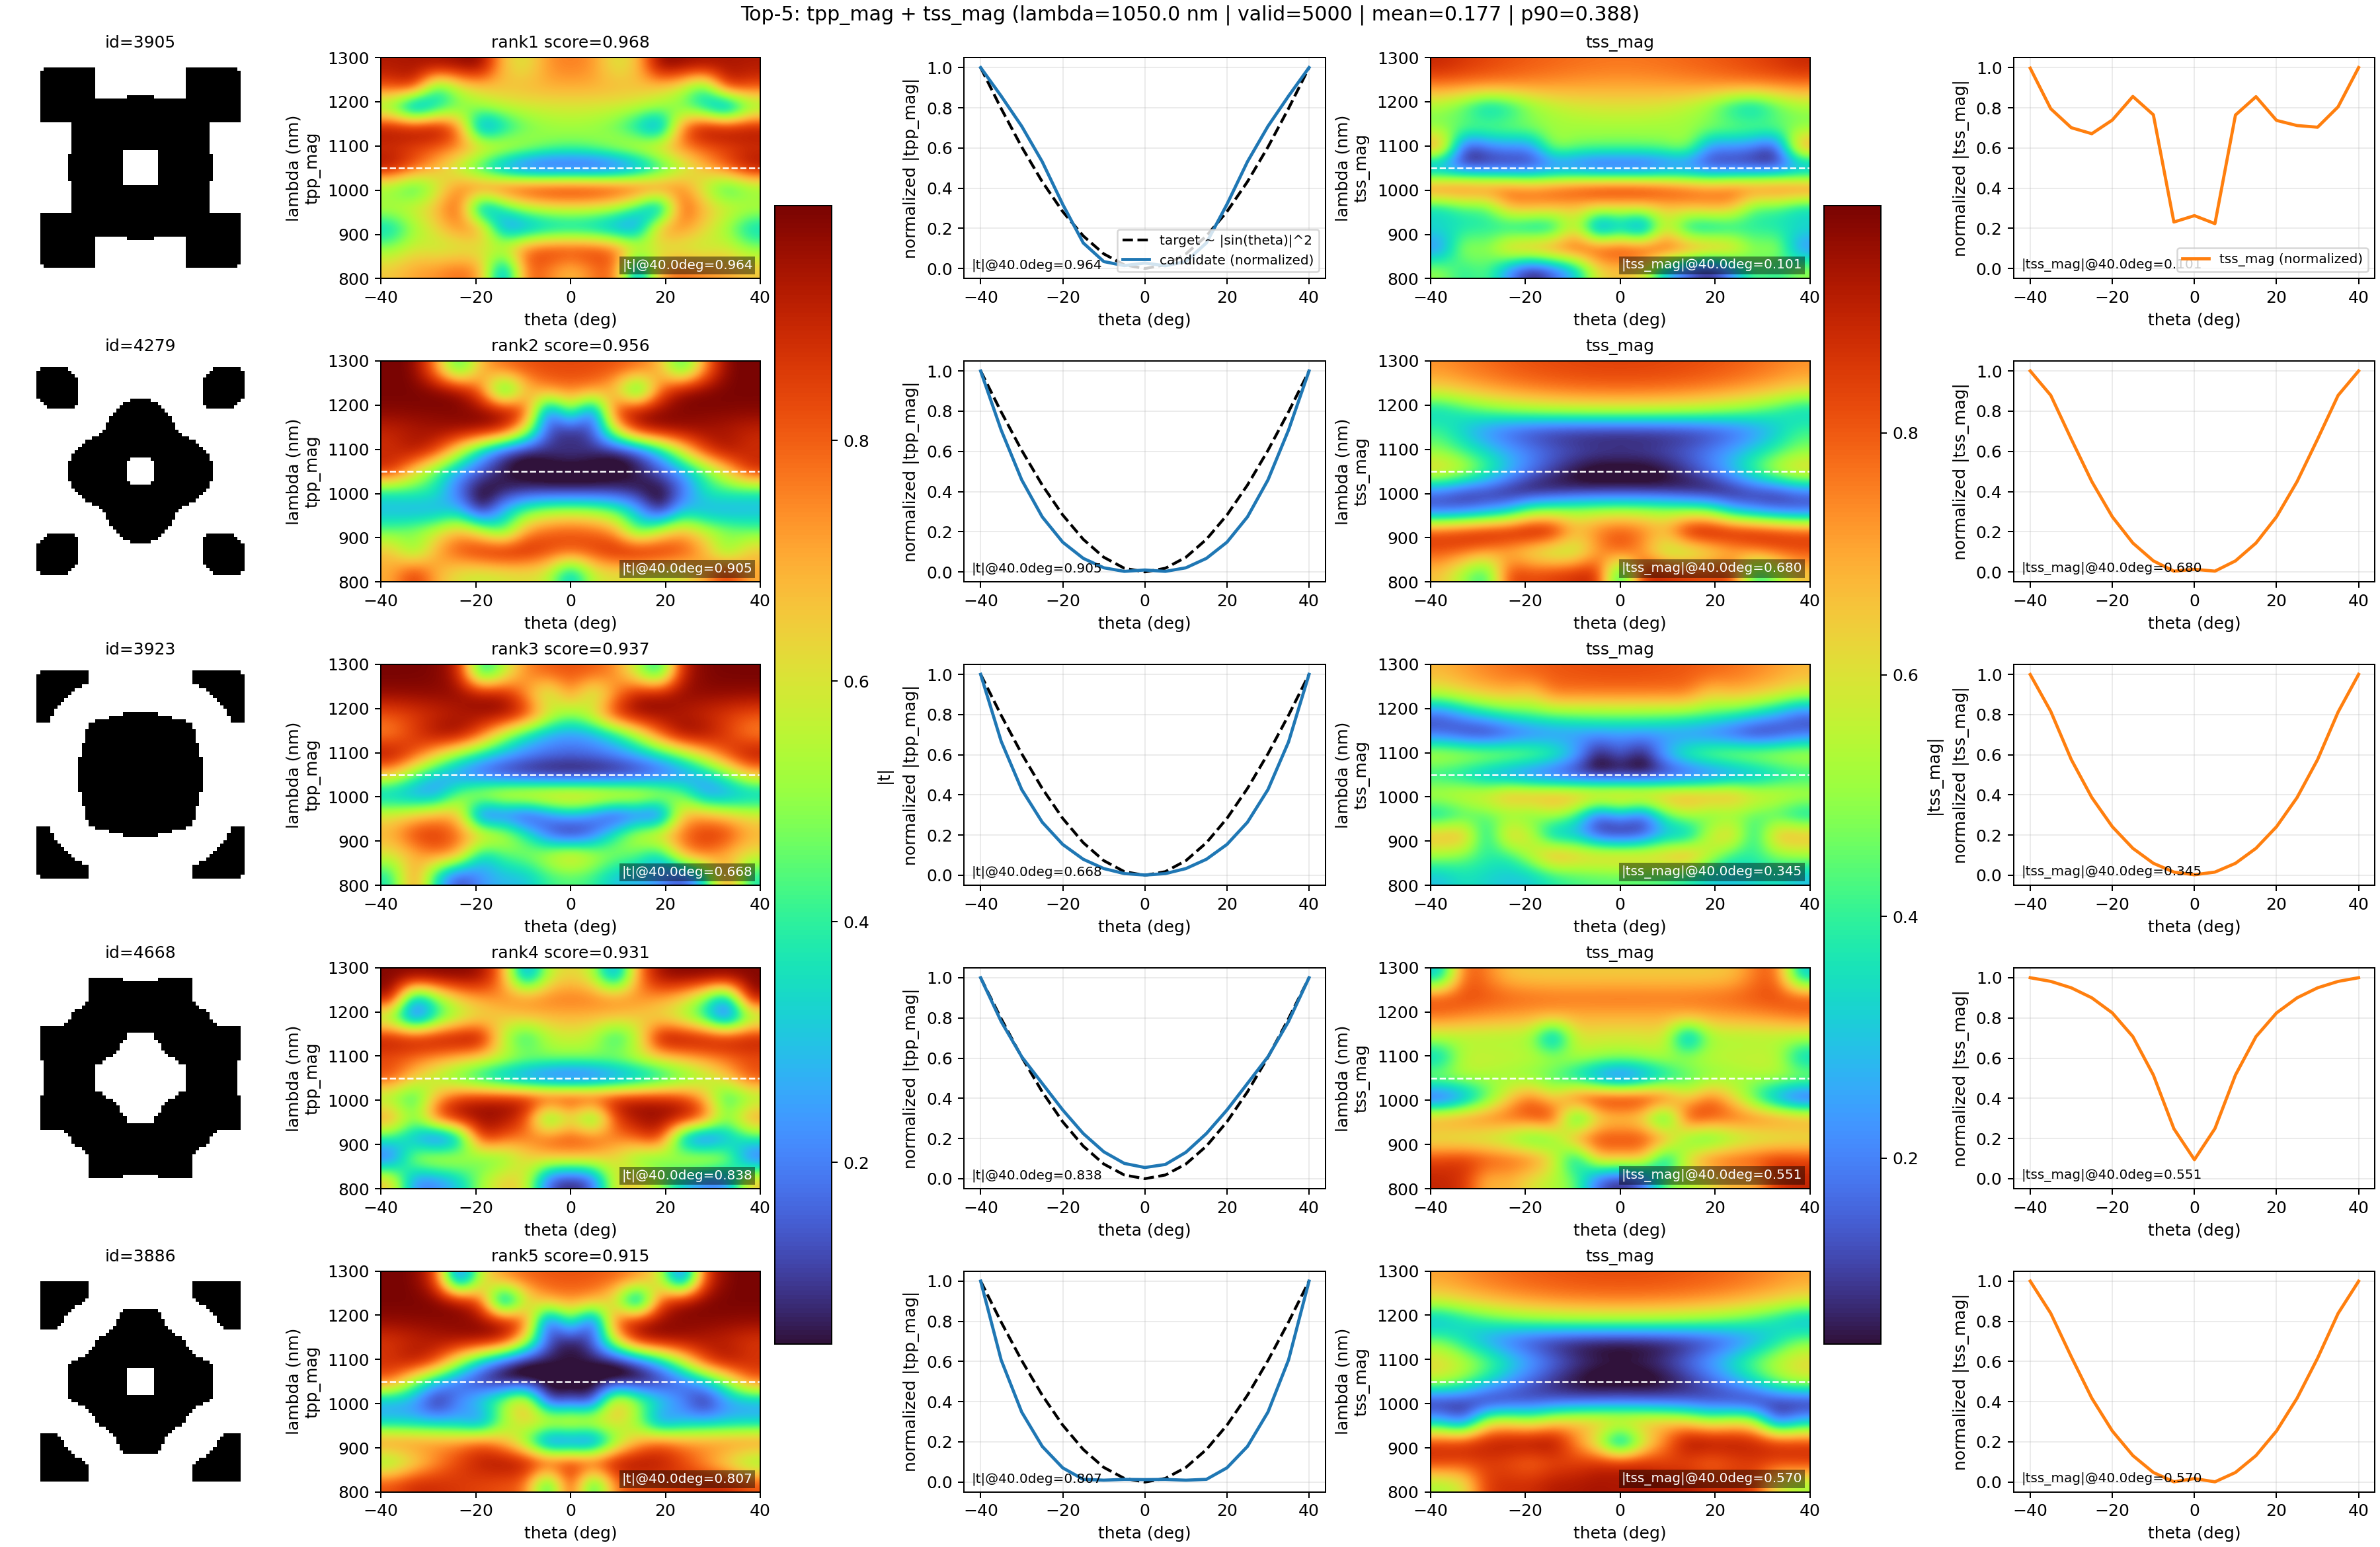
\includegraphics[width=0.78\linewidth]{../data/second_order_scores/tpp_mag_top5_plots/lambda_1050.0nm_top5.png}
\caption{Top ranked second-order candidates at 1050~nm. The ranking overview visualizes the concentration of operator-like responses that motivates task-aware simulation-based reranking.}
\label{fig:second1050}
\end{figure}

Figure~\ref{fig:second1050} shows the top-five ranking overview at 1050~nm, where the leading candidate already displays a representative second-order response. The result is more than a ``high score by normalization.'' It preserves the expected second-order envelope over a wide angular aperture and therefore remains meaningful under operator-level interpretation. The recurrence of closely related high-performing responses across independent evaluations suggests that the best second-order devices occupy especially stable regions of the verified response manifold.

The second-order case also supports the strongest literature-level positioning. Under the same downstream imaging analysis used throughout this study, the best 1050~nm result is associated with a normalized task score of about $0.988$, a relative edge amplitude ratio near $0.97$, an effective working bandwidth around $100$~nm, and a numerical aperture around $0.64$. These numbers place the design in the same performance conversation as recent broadband, high-NA, high-efficiency differentiator reports \cite{cotrufo2023natcom,deng2024,qiu2025highorder,zhou2025laplace}. The precise contribution of the present work, however, is different from a single-device record chase: the same response-centered framework produces this high-performing second-order behavior and also extends naturally to polarization and spatiotemporal targets.

\begin{figure}[!htbp]
\centering
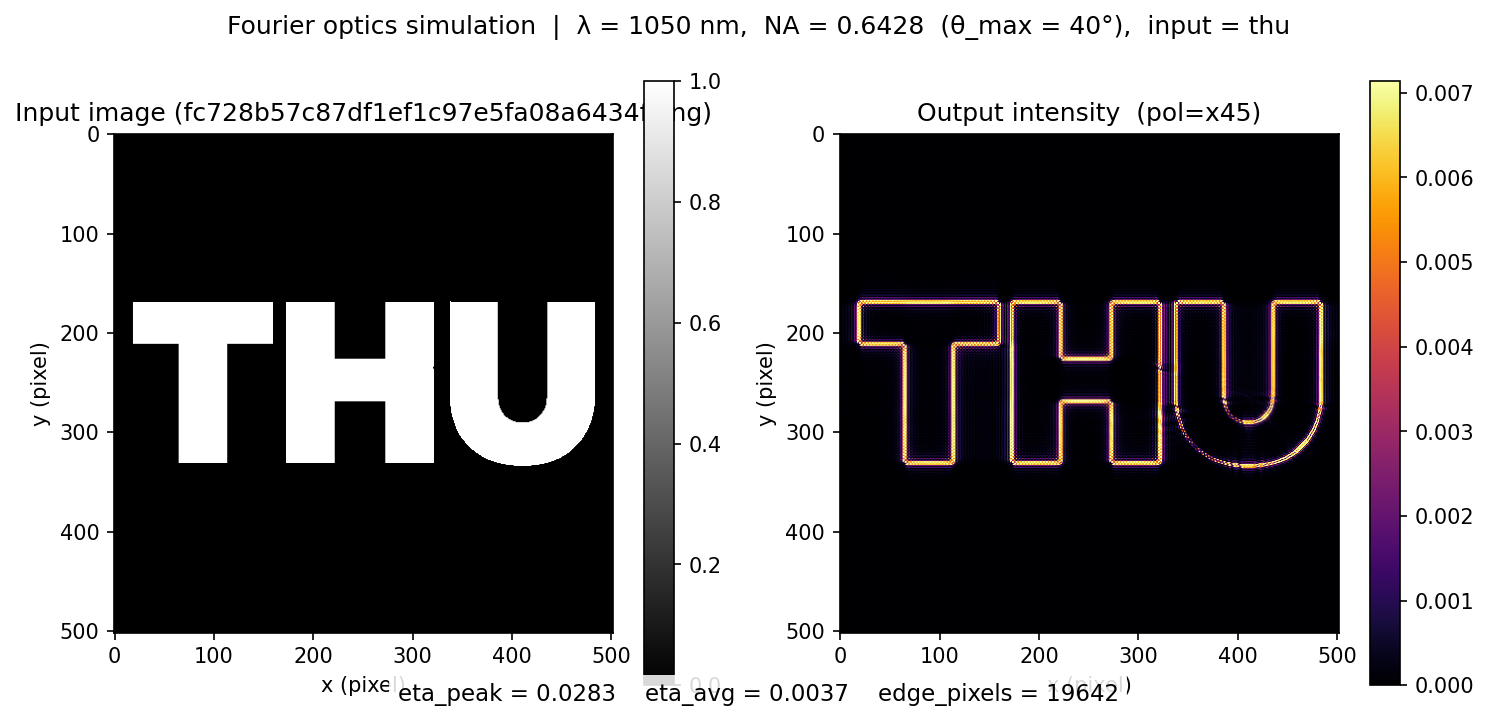
\includegraphics[width=0.63\linewidth]{../src/infer/results/p/1050nm_id4279/run_imaging_p_1050nm_id4279_1050nm_from_kspace_x45_thu_20260405_162600/imaging_result.png}
\caption{Image-domain validation for the leading 1050~nm second-order result. The response-level agreement translates into practical edge-enhancement behavior rather than remaining a numerical score gain only.}
\label{fig:imaging}
\end{figure}

Figure~\ref{fig:imaging} closes the argument by moving from response space to image space. Once the verified transfer function is inserted back into the Fourier imaging pipeline, the resulting output exhibits the expected second-derivative effect: low-frequency regions are suppressed while edge-like features and curvature-sensitive structures are enhanced. This is the key bridge between operator scoring and practical device function. The inverse-design loop is successful because a physically verified structure reproduces both the target response geometry and its intended optical action.

\begin{table}[!htbp]
\centering
\caption{Representative verified results used throughout the paper. Scores reflect task-specific rankings rather than abstract model confidence.}
\label{tab:cases}
\begin{tabular}{>{\raggedright\arraybackslash}p{3.3cm}c>{\raggedleft\arraybackslash}p{2.2cm}>{\raggedleft\arraybackslash}p{4.1cm}}
\toprule
Task & $\lambda$ (nm) & Main score & Notes \\
\midrule
Second-order & 1050 & 0.9306 & representative $T_{pp}$ response with large NA and high transmission \\
Second-order & 1100 & 0.9308 & strongest verified 1100~nm result \\
Polarization independent & 1000 & 0.9358 & matched dual-channel operator response \\
Polarization multiplexed & 1100 & 0.7283 & active score $0.9348$ with passive suppression retained \\
Fourth-order & 1150 & 0.8884 & sharp outer-angle growth \\
Low-pass & 1050 & 0.9934 & strongest passband-shaping result \\
Spatiotemporal window & 950 & 0.7271 & strongest merged window score in the verified screen \\
\bottomrule
\end{tabular}
\end{table}

\FloatBarrier

\subsection{Generalization to other OTF targets}

The most important question after this second-order result is whether the same response-centered loop continues to behave coherently when the target shape changes. The verified results give a positive answer across three independent axes.

The first axis is polarization. In the polarization-independent benchmark, the best 1000~nm result reaches a joint verified score of $0.9358$, while the leading 1050 and 1100~nm results remain above $0.88$ and $0.91$, respectively. This matters because the task score does not merely average two channels: it rewards channel-wise operator fidelity and explicit amplitude agreement around $\pm40^{\circ}$. The fact that the same framework can produce matched $T_{pp}$ and $T_{ss}$ operator responses shows that polarization enters naturally as a first-class conditioning axis.

The second axis is polarization multiplexing. The strongest verified multiplexed result at 1100~nm reaches a joint score of $0.7283$, together with an active-channel operator score of $0.9348$ and a passive-channel suppression term of $0.5218$. In other words, the framework learns to preserve operator shape while also distinguishing which channel should carry the response and which should remain as silent as possible. This is exactly the kind of channel-level tradeoff that a unified response tensor should expose.

\begin{figure}[!htbp]
\centering
\begin{minipage}[t]{0.48\linewidth}
\centering
\includegraphics[width=\linewidth]{../data/polarization_independent_scores/joint_top1_plots/lambda_1000.0nm_top1.png}
\end{minipage}\hfill
\begin{minipage}[t]{0.48\linewidth}
\centering
\includegraphics[width=\linewidth]{../data/polarization_multiplexed_scores/p_active_s_silent/p_active_s_silent_top5_plots/p_active_s_silent_lambda_1100.0nm_top5.png}
\end{minipage}
\caption{Polarization-aware generalization. Left: polarization-independent top case at 1000~nm. Right: polarization-multiplexed top candidates at 1100~nm. The same inverse-design loop can either align the two channels or intentionally separate them.}
\label{fig:pol}
\end{figure}

The third axis is target-shape diversity. In the fourth-order benchmark, the 1050~nm response family reaches a top score of $0.9222$, while the strongest verified 1150~nm result reaches $0.8884$. These values indicate that the framework remains effective even when the desired response becomes sharper than a second-order bowl. In the low-pass benchmark, the best verified results reach $0.9934$ at 1050~nm and $0.9863$ at 1100~nm, demonstrating that the same tensor-conditioning strategy can realize a fundamentally different angular envelope in addition to polynomial-like operator responses.

Spatiotemporal targets provide the strongest stress test because they are evaluated on a two-dimensional wavelength--angle window instead of a single wavelength row. The dataset-level screen at 950~nm identifies a top merged score of $0.7271$, which is already meaningful given the difficulty of jointly controlling the central zero lines and the corner lobes of the ideal map. This confirms that the response-window view is not merely rhetorical, but remains quantitatively meaningful under the same verified ranking logic.

\begin{figure}[!htbp]
\centering
\begin{minipage}[t]{0.48\linewidth}
\centering

\includegraphics[width=\linewidth]{../data/optica_lowpass_scores/tpp_mag_optica_lowpass_top5_plots/lambda_1050.0nm_top5.png}
\end{minipage}\hfill
\begin{minipage}[t]{0.48\linewidth}
\centering
\includegraphics[width=\linewidth]{../data/st2_template_match_20260330_233804/lambda_950nm/rank_001_sample_5409.png}
\end{minipage}
\caption{Generalization beyond second-order differentiation. Left: low-pass target at 1050~nm. Right: top spatiotemporal candidate at 950~nm from the wavelength--angle window ranking pipeline.}
\label{fig:generalization}
\end{figure}

Taken together, Figures~\ref{fig:pol} and~\ref{fig:generalization} support the same conclusion. The present method goes beyond a differentiator-specific recipe. It forms a unified response-space design loop that can absorb changes in channel requirements, target curvature, target envelope, and even in the dimensionality of the target support.

\FloatBarrier

\subsection{Model comparison and evaluation protocol}

A unified comparison protocol is defined for topology optimization, CVAE, cGAN, and diffusion under the same target condition and the same simulation-based post-verification metrics. The shared evaluation reports best score, mean score, top-3 score, success rate above threshold, spectrum MAE, binary rate, diversity, and inference time. This is the correct comparison language for the present problem because a strong inverse designer should hit good samples consistently and should also populate the feasible set with diverse physically useful candidates.

At the current stage of the study, the retained checkpoints directly support the forward surrogate and the physics-guided diffusion pipeline, whereas the cVAE and cGAN baselines and the topology-optimization branch are not all accompanied by synchronized checkpoints. Table~\ref{tab:compare} therefore serves two purposes. It makes the quantitative protocol explicit and it records only the directly available evidence without fabricating missing baseline numbers.

\begin{table}[!htbp]
\centering
\caption{Comparison protocol used in this study. The metrics are computed after full-wave verification. Quantitative training endpoints are listed only where directly retained evidence is available.}
\label{tab:compare}
\begin{tabular}{>{\raggedright\arraybackslash}p{2.1cm}>{\raggedright\arraybackslash}p{2.4cm}>{\raggedleft\arraybackslash}p{2.1cm}>{\raggedleft\arraybackslash}p{2.1cm}}
\toprule
Method & Condition / objective & Direct retained evidence & Status \\
\midrule
Forward surrogate & structure $\rightarrow$ response, normalized $L_1$ & val loss $\approx 0.366$ & checkpoint + log retained \\
Diffusion & response $\rightarrow$ structure, diffusion + physics + binary losses & val loss $\approx 0.129$ & checkpoint + log retained \\
CVAE & response $\rightarrow$ structure, variational baseline & unified eval supported & checkpoint absent locally \\
cGAN & response $\rightarrow$ structure, adversarial baseline & unified eval supported & checkpoint absent locally \\
Topo-opt & task-guided iterative search & unified eval supported & legacy dependency incomplete locally \\
\bottomrule
\end{tabular}
\end{table}

Even with this limitation, the comparison section remains scientifically useful. The evaluation protocol already formalizes the right question: the inverse method should be judged by verified best-case score, average candidate quality, response MAE, binarity, and diversity under shared targets. The present physics-guided diffusion pipeline is the only branch for which the end-to-end checkpointed evidence is directly retained, which is why it becomes the center of the manuscript.

\section{Discussion}

The first point worth emphasizing is a scaling-law trend. In the present study, performance improves as the verified dataset grows from the 1\,000-sample level to the $2\times10^4$ level, and it also benefits from stronger surrogate and generative backbones. In that sense, the present results already provide an initial scaling-law signal of their own. The analogy to empirical scaling laws in large language models is suggestive rather than literal \cite{kaplan2020scaling}: once the target is a structured wavelength--angle--polarization field, success depends on how well the model sees rare but valuable response modes and how accurately the forward surrogate resolves them. The main limitation is that the current scaling axis is still narrow, since the framework so far fixes the material platform, lattice period, and amplitude-only response representation. A natural next step is therefore to scale not only dataset size and model capacity, but also the physical design space itself, by incorporating multiple material systems, variable periods, and phase-sensitive targets into the same response-centered formulation. If those axes can be enlarged together with denser electromagnetic verification, the framework may evolve toward a more general metasurface inverse-design regime.

The second point is the extensibility of the design space itself. Because the target is written as a response tensor rather than a single scalar objective, the same framework can in principle be extended toward joint polarization--frequency--angle design, where multiple physical channels are shaped simultaneously. This broader setting is relevant to compact folded and angle-resolved spectrometers \cite{faraji2018folded,cai2024angleresolved}, multidimensional sensing and computational photodetection \cite{jiang2024multidimensional}, and polarization-encoded information or optical encryption devices \cite{guo2022stokes}. In that sense, the present work is better viewed as a general response-level design methodology than as a closed list of six isolated examples.

\section{Conclusion}

This paper has rewritten freeform Fourier-operator metasurface design as a response-centered inverse problem defined over wavelength, angle, and polarization. On that basis, it develops a coherent physical loop comprising fabrication-aware structure generation, simulation-based labeling, score-aware data preparation, forward surrogate training, conditional diffusion sampling, and simulation-based reranking. The key scientific point is that the optical target should be specified in the same response space in which the final device is verified, placing the present study in closer contact with objective-driven photonic inverse design and response-faithful electromagnetic modeling \cite{an2019deep,ma2019probabilistic,phillips2021ensemble}.

Within this formulation, a second-order differentiator with large NA, high transmission, and broadband operation reaches a leading level of verified performance across multiple wavelengths, while polarization-independent, polarization-multiplexed, fourth-order, low-pass, and spatiotemporal targets can likewise be handled at a competitive level within the same unified inference framework. The broader contribution is the demonstration that multiple operator families can be described, generated, and judged within one physically consistent design language.

The broader implication is methodological. Freeform metasurface inverse design is better treated as target-conditioned feasible-set discovery under electromagnetic verification than as single-geometry regression or task-label prediction detached from the transfer function. The present study provides one concrete realization of that principle, and it points naturally toward future extensions involving richer polarization control, full complex-response targets, broader physical design spaces, tighter fabrication models, and larger-scale physics-guided datasets.


% ===== References =====
\bibliographystyle{unsrt}
\bibliography{refs}

\end{document}
